The proposed ontology workflow uses alphanumeric identifiers in order to adhere to the development rules described in Section~\ref{ssec:development-rules}. These numerical identifier encode two pieces of information: A unique id for the given entity and the developer that added this entity.

Alphanumeric identifiers are listed as best
practice and commonly used because in most cases their advantages
outweigh the disadvantages. A short summary is given below:
\paragraph{Advantages} 
\begin{itemize}
    \item Versioning and backward compatibility: A name for a concept
    can change in a new version of the ontology without its identifier (in
    databases etc.) having to be changed everywhere. 
    \item User groups: If people
    talk about the same concept but can't decide on a main name for it, they
    can both be added as labels for this concept and the people can get
    their own views of the ontology showing their preferred label. 
    \item Better readability: In labels, we do not have to use CamelCase. Long names like NonRenewableMunicipalWasteFuel are better readable in lower case as ``non renewable municipial waste fuel''.
\end{itemize}


\hypertarget{disadvantages}{%
\paragraph{Disadvantages}\label{disadvantages}}

\begin{itemize}
\item
  The file is harder to read without a tool like Prot\'eg\'e (that will
  automatically show labels instead of the alphanumerical identifiers).
\end{itemize}


\subsubsection{List of user ID's}
\label{ssec:list-of-user-ids}

The list of user ids can be found in the main ontology file. The ID's got added in front of the \emph{dc:contributor}
annotation of the person they belong to. New developers can add themself via a pull request.


\subsubsection{Implementation in the Template Ontology}\label{sssec:implementation-in-the-mno}

Identifiers look like this: MNO\_00010123

They are structured in three parts: {[}Ontology{]}\_{[}yyyy{]}{[}xxxx{]}
\begin{itemize}
    \item ``{[}Ontology{]}\_'' identifies the ontology that this class belongs to. 
    \item {[}yyyy{]} identifies the user who added the classes. Each user gets a unique ID.
    \item {[}xxxx{]} identifies the
specific class added by the user. 
\end{itemize}

This enables every user to create 10000 entities before having to get a new ID. IDs are assigned chronologically to each entity, starting with 0000.


\subsubsection{How to change your
settings}
\label{sssec:how-to-change-your-settings}

Protege is able to generate these IRIs automatically, but the required settings are not entirely intuitive. Navigate to \textit{$\text{File}\rightarrow\text{Preferences}\rightarrow\text{New Entities}$} and change the following settings. 

\begin{figure}
    \centering
    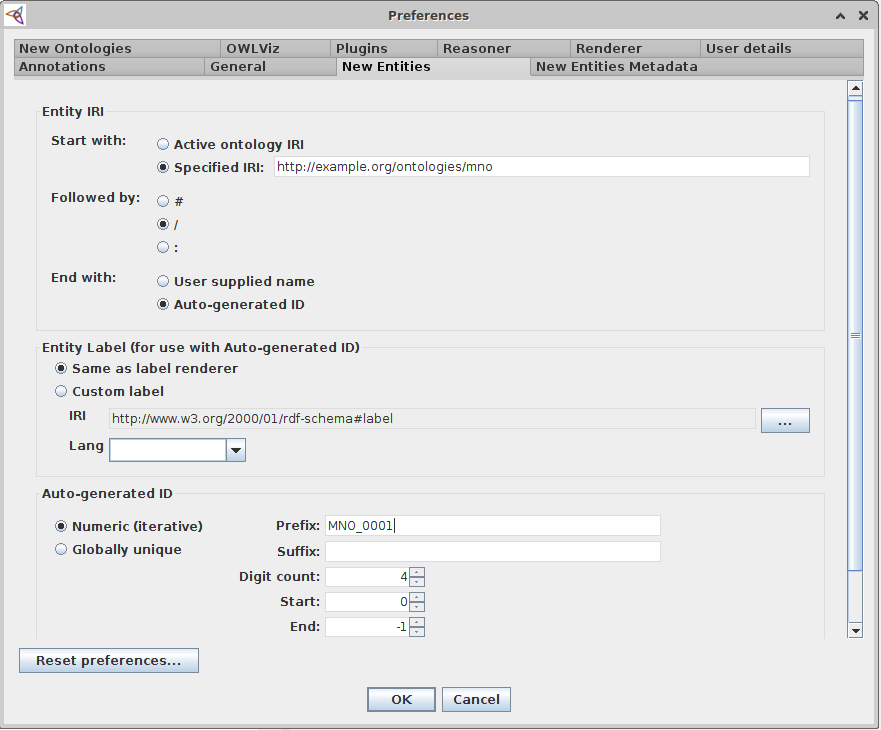
\includegraphics[width=\textwidth]{fig/protege-settings.png}
    \caption{Settings in \textit{$\text{File}\rightarrow\text{Preferences}\rightarrow\text{New Entities}$} as described in Section \ref{sssec:implementation-in-the-mno}.}
    \label{fig:protege-settings}
\end{figure}

\begin{itemize}
    \item \texttt{Entity\ IRI:}
    \begin{itemize}
        \item \texttt{Starts with:} Select the \texttt{Specific\ IRI} option and change it to the Ontology IRI of your ontology
        \item \texttt{Followed by:} This setting depends on how the IRIs are resolved.
        \item \texttt{Ends with:} Select the \texttt{Auto-generated\ ID} option\todo{Explain settings}
    \end{itemize}
\item \texttt{Entity Label:} Choose the \texttt{Same as label renderer} option
\item \texttt{Auto-generated ID:}  Choose the \texttt{Numeric (iterative)} option and set the following parameters
\begin{itemize}
    \item \texttt{Prefix:} [Ontology]\_{[}your user id{]} e.g. MNO\_0001 if you user ID is 1
    \item \texttt{Digit count:} The number of digits that your entity identifiers should have.
    \item \texttt{Start:} The smallest value for entity identifiers
    \item \texttt{End:} The largest possible value for entity identifiers
\end{itemize}
\end{itemize}
An example for these settings is shown in Figure~\ref{fig:protege-settings}.
